\section{Nernst-Planck, a special case}
This benchmark aims to test the advection due to present electrical
fields in the advection diffusion solver. It is done by solving for
the ion concentration in a system that fulfils the assumptions for the
Poisson-Boltzmann distribution. Beside a system in steady state, the
assumptions are a simple geometry that allows for the one dimensional
integration and a zero advective velocity, see section
\ref{sec:et:pb}. 

A 1:1 ion solution will be considered and therefore two solvers for
the Nernst-Planck equation are needed. One for positive and one for
negative ions. These will be coupled to a solver for Poisson's
equation which will update the potential each time step according to
the present ion concentration. In the steady state, the ion
concentrations for positive and negative ions respectively are
compared to the exponential expression in the Poisson-Boltzmann
situation, eq. \eqref{eq:C}. The potential in this expression is
obtained by solving the Poisson-Boltzmann equation,
eq. \eqref{eq:pb_real}.


Two solvers using the method in section, \ref{sec:lbm:np} are set up
with the following set of parameters:

\begin{itemize}
\item[] z = $\pm$ 1
\item[] D = $10^{-8}$ m$^2$s$^{-1}$
\item[] T = 293 K
\item[] $\epsilon_r$ = 80
\end{itemize}
The Nernst-Planck equation is put on non-dimensional form by
introducing the following characteristic quantities:

\begin{itemize}
\item[] $\cnil$ = $10^{-4}$ mol/m$^3$
\item[] $\lnil$ = 2$\cdot10^{-5}$/ny m
\item[] $\Vnil$ = -50 mV
\item[] $\unil$ = 0.1 m/s.
\end{itemize}
These parameters gives a Peclet number of $\Pe = 2$ which gives a
relaxation parameter $\omega_{NP} = 0.5$.

The geometry of the system simulated is an infinite channel with
straight walls. A grid of 3$\times$100 nodes is used for the
computation, i.e. 100 nodes across the channel. At the walls, the no
flux boundary condition, eq. \eqref{eq:et:j0}, is implied through the
mirror reflection approach described in section,
\ref{sec:lbm:mirror}. For the Poisson solver, a constant surface
charge density of $\sigma = -0.17$ $\mu$C/m$^2$ is applied to the
walls, eq. \eqref{eq:et:fix_c}. This is realised by a modified mirror
reflection, see section \ref{sec:lbm:mod_mirror}.

The charge concentration at the middle of the channel (denoted by
$\C^{\infty}$ in eq. \eqref{eq:C}) in the Poisson-Boltzmann distribution
are set to the values obtained from the Nernst-Planck solver. 

In fig. \ref{fig:mb:np}, the resulting charge distributions are
presented.  

\begin{figure}
\begin{center}
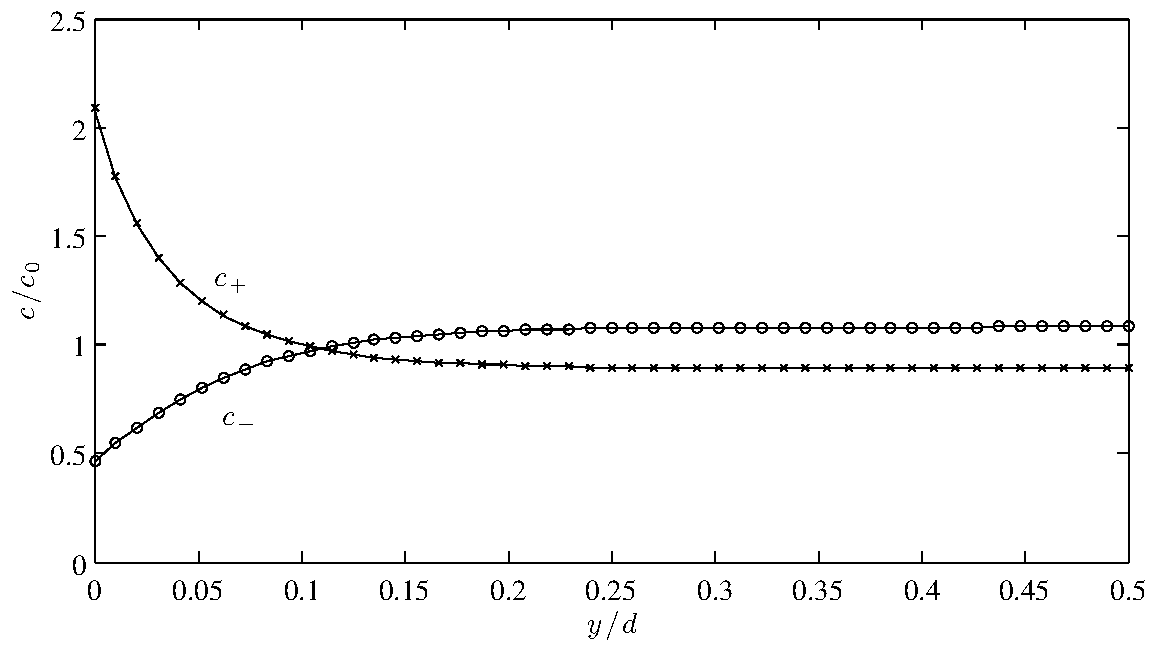
\includegraphics[width=0.9\textwidth]{fig/np_bench.pdf}
\end{center}
\caption{Computed charge concentrations for positive ($\C_+$) and
  negative ($\C_{-}$) ions respectively in contact with a negatively
  charged wall. The concentrations are compared with the
  Poisson-Boltzmann distribution (solid).}
\label{fig:mb:np}
\end{figure}


